% ===========================================================================
% Part VII - Unsupervised Neural Learning: Self-Organizing Maps (Experiment 15)
% ===========================================================================

\part{Unsupervised Neural Learning: Self-Organizing Maps}

% ---------------------------------------------------------------------------
\chapter{Experiment 15: Self-Organizing Map (SOM)}\label{exp:15}

\quickfacts
  {Dataset}{UCI Wine: 178 samples, 13 chemical features, 3 cultivars (labels used only for visualization)}
  {Key parameters}{12$\times$12 grid, Gaussian neighborhood, $\sigma$ = 1.5, learning rate 0.5, PCA initialization, 5,000 iterations}
  {Headline result}{Quantization error 0.4447 $\rightarrow$ 0.1965; topographic error 0.0393}

\section{Objective}
Use a Self-Organizing Map to map high-dimensional observations onto a low-dimensional grid
while preserving neighborhood structure.

\section{Suggested Dataset}
UCI Wine: 178 samples, 13 chemical features, 3 cultivars (labels used only for
visualization). Features are MinMax-scaled to $[0, 1]$.

\section{Required Libraries}
minisom, numpy, pandas, matplotlib.

\section{Brief Theory}
A Self-Organizing Map is a grid of neurons, each with a weight vector $w_j$ in the input
space. For each training sample the algorithm performs three steps:
\begin{enumerate}
  \item \textbf{competition:} find the Best Matching Unit
        $c = \arg\min_j \lVert x - w_j \rVert$;
  \item \textbf{cooperation:} compute the Gaussian neighborhood
        $h_{cj}(t) = \exp\!\bigl(-\lVert r_c - r_j\rVert^2 / (2\sigma(t)^2)\bigr)$
        on grid coordinates $r$;
  \item \textbf{adaptation:} move the weights toward the input,
        $w_j \leftarrow w_j + \alpha(t)\,h_{cj}(t)\,(x - w_j)$.
\end{enumerate}
The learning rate $\alpha(t)$ and radius $\sigma(t)$ decay over time: early large neighborhoods
organize the global layout, later small updates refine details. The result is a
topology-preserving 2D projection. Quality is measured by the \textbf{quantization error}
(average distance from samples to their BMU) and the \textbf{topographic error} (fraction of
samples whose two best neurons are not neighbors). The \textbf{U-matrix} visualizes cluster
boundaries as ridges of high inter-neuron distance.

\section{Procedure}
\begin{enumerate}
  \item Load the wine data and MinMax-scale to $[0, 1]$.
  \item Create a 12$\times$12 SOM with a Gaussian neighborhood ($\sigma = 1.5$, learning rate
        0.5) and initialize the weights with PCA.
  \item Train for 5,000 random samples.
  \item Compute the quantization and topographic errors.
  \item Plot the U-matrix with each sample projected onto its BMU (marker = true cultivar).
  \item Discuss grid size and $\sigma$.
\end{enumerate}

\section{Reference Implementation}
\begin{lstlisting}[style=mlcode,caption={Creating, initializing and training the Kohonen map}]
som = MiniSom(x=12, y=12, input_len=13, sigma=1.5, learning_rate=0.5,
              neighborhood_function='gaussian', random_seed=42)
som.pca_weights_init(X)
som.train_random(data=X, num_iteration=5000)
qe = som.quantization_error(X); te = som.topographic_error(X)
\end{lstlisting}

\section{Evaluation / Expected Output}
\begin{table}[htbp]
  \centering
  \caption{SOM quality metrics on the Wine data.}
  \begin{tabular}{@{}lr@{}}
    \toprule
    \textbf{Metric} & \textbf{Value} \\
    \midrule
    Initial quantization error & 0.4447 \\
    Final quantization error & \best{0.1965} \\
    Topographic error & \best{0.0393} ($\approx$ 4\% foldings) \\
    \bottomrule
  \end{tabular}
\end{table}

\begin{figure}[htbp]
  \centering
  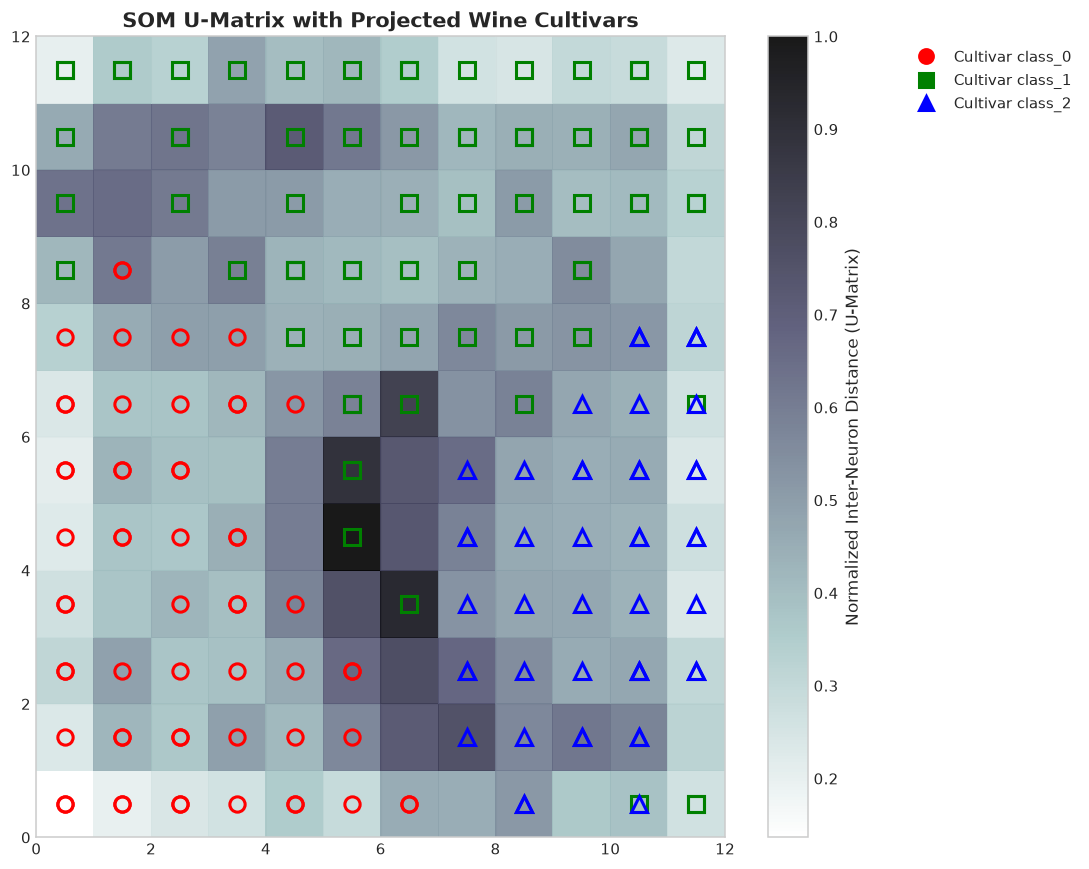
\includegraphics[width=0.85\textwidth]{figures/exp15_umatrix.png}
  \caption{SOM U-matrix with the wine samples projected onto their BMUs; marker shape and
  color encode the true cultivar.}
  \label{fig:exp15-umatrix}
\end{figure}

The map halved its quantization error during training and preserves topology well (topographic
error below 0.05). On the U-matrix the three wine cultivars occupy contiguous regions separated
by bright ridges, even though the SOM never saw the labels --- evidence of unsupervised
structure discovery. PCA initialization gave a well-unfolded map from the start.

\section{Viva / Discussion Questions}
\begin{description}
  \item[SOM vs K-means?] Both compress data with prototypes, but K-means only finds centroids
  while SOM arranges them on a grid so neighboring neurons represent similar inputs (topology
  preservation).
  \item[What is a BMU?] The neuron whose weight vector is closest to the input --- the winner
  of the competition.
  \item[Why is SOM called a topology-preserving map?] The neighborhood update ensures nearby
  grid positions end up with similar weight vectors, so high-dimensional neighborhoods are
  approximately preserved in 2D.
  \item[Why initialize with PCA?] Random initialization can create folded maps; PCA starts the
  map spread along the data's principal directions, giving faster and more faithful
  convergence.
\end{description}

\section{Complete Code Listing}
% ===========================================================================
% exp15_som.tex - complete code listings for Experiment 15
% Source: notebooks/07_self_organizing_map.ipynb (executed)
% Repository: https://github.com/Atik203/ML-Algorithms
% ===========================================================================

\begin{codebox}[title={Core numerical and plotting libraries}]
# ---- Core numerical and plotting libraries ----
import numpy as np
import pandas as pd
import matplotlib.pyplot as plt
import seaborn as sns

# ---- Dataset + scaling ----
from sklearn.datasets import load_wine
from sklearn.preprocessing import MinMaxScaler
# ---- MiniSom: lightweight Kohonen Self-Organizing Map implementation ----
from minisom import MiniSom

# Styling setup (consistent look across all notebooks)
plt.style.use('seaborn-v0_8-whitegrid' if 'seaborn-v0_8-whitegrid' in plt.style.available else 'default')
plt.rcParams['font.sans-serif'] = 'DejaVu Sans'
plt.rcParams['figure.figsize'] = (10, 6)
plt.rcParams['figure.dpi'] = 110

np.random.seed(42)
print("MiniSom and libraries loaded successfully!")

# ---- Load the Wine recognition dataset ----
wine = load_wine()
X_raw = wine.data          # 178 samples x 13 chemical features
y = wine.target            # 3 wine cultivars (only used for visualization - SOM is unsupervised)
feature_names = wine.feature_names
target_names = wine.target_names

print(f"Samples: {X_raw.shape[0]}, Features: {X_raw.shape[1]}, Classes: {target_names.tolist()}")

# ---- MinMax scaling to [0, 1] ----
# SOM weight vectors live in the same range as the inputs, so scaling keeps learning stable.
scaler = MinMaxScaler()
X = scaler.fit_transform(X_raw)
\end{codebox}

\begin{codebox}[title={Configure the Kohonen grid}]
# ---- Configure the Kohonen grid ----
grid_x, grid_y = 12, 12  # 12x12 grid = 144 neurons (fewer than the 178 samples)
input_len = X.shape[1]   # 13 chemical features per neuron weight vector

som = MiniSom(
    x=grid_x,
    y=grid_y,
    input_len=input_len,
    sigma=1.5,                       # initial neighborhood radius
    learning_rate=0.5,               # initial learning rate
    neighborhood_function='gaussian',# smooth Gaussian neighborhood kernel
    random_seed=42
)

# ---- Initialize weights with PCA for topologically faithful, faster convergence ----
som.pca_weights_init(X)
print("Initial Quantization Error:", som.quantization_error(X))

# ---- Train: 5000 random samples presented to the map ----
som.train_random(data=X, num_iteration=5000, verbose=False)
final_qe = som.quantization_error(X)   # average distance from samples to their BMU
final_te = som.topographic_error(X)    # fraction of samples whose 2nd BMU is not a grid neighbor

print(f"Training complete after 5,000 iterations!")
print(f" - Final Quantization Error (mean distance to BMU): {final_qe:.4f}")
print(f" - Final Topographic Error (proportion of foldings): {final_te:.4f}")
\end{codebox}

\begin{codebox}[title={Plot the U-Matrix (unified distance map)}]
# ---- Plot the U-Matrix (unified distance map) ----
# Each cell = average distance between a neuron and its immediate grid neighbors.
# Dark valleys = dense clusters; bright ridges = boundaries between clusters.
plt.figure(figsize=(10, 8))
plt.pcolor(som.distance_map().T, cmap='bone_r', alpha=0.9)
cbar = plt.colorbar()
cbar.set_label("Normalized Inter-Neuron Distance (U-Matrix)", fontsize=11)

# ---- Project every sample onto its Best Matching Unit (BMU) ----
markers = ['o', 's', '^']
colors = ['red', 'green', 'blue']

for idx, x_vec in enumerate(X):
    w = som.winner(x_vec)  # grid coordinates of the best matching neuron for this sample
    plt.plot(
        w[0] + 0.5,        # +0.5 centers the marker inside the pcolor cell
        w[1] + 0.5,
        markers[y[idx]],   # marker shape encodes the true cultivar
        markerfacecolor='None',
        markeredgecolor=colors[y[idx]],
        markersize=10,
        markeredgewidth=2
    )

# Build a legend for the three cultivars
for c_idx, c_name in enumerate(target_names):
    plt.plot([], [], marker=markers[c_idx], color=colors[c_idx], linestyle='None',
             label=f'Cultivar {c_name}', markersize=9, markeredgewidth=2)

plt.title("SOM U-Matrix with Projected Wine Cultivars", fontsize=14, fontweight='bold')
plt.legend(bbox_to_anchor=(1.25, 1), loc='upper left')
plt.tight_layout()
plt.show()
\end{codebox}

